%! BibTeX Compiler = bibtex
%TC:ignore
\documentclass{article}
\usepackage{caption}
\usepackage{xcolor, colortbl}
\definecolor{BLUELINK}{HTML}{0645AD}
\definecolor{DARKBLUELINK}{HTML}{0B0080}
\definecolor{LIGHTGREY}{gray}{0.9}
\PassOptionsToPackage{hyphens}{url}
\usepackage[colorlinks=false]{hyperref}
% for linking between references, figures, TOC, etc in the pdf document
\hypersetup{colorlinks,
    linkcolor=DARKBLUELINK,
    anchorcolor=DARKBLUELINK,
    citecolor=DARKBLUELINK,
    filecolor=DARKBLUELINK,
    menucolor=DARKBLUELINK,
    urlcolor=BLUELINK
} % Color citation links in purple
\PassOptionsToPackage{unicode}{hyperref}
\PassOptionsToPackage{naturalnames}{hyperref}

\usepackage{biorxiv}

\usepackage{url}
\usepackage{amssymb,amsfonts,amsmath,amsthm,mathtools}
\usepackage{lmodern}
\usepackage{xfrac, nicefrac}
\usepackage{bm}
\usepackage{listings, enumerate, enumitem}
\usepackage[export]{adjustbox}
\usepackage{graphicx}
\usepackage{bbold}
\usepackage{pdfpages}
\pdfinclusioncopyfonts=1
\usepackage{lineno}
\usepackage{tabu}
\usepackage{hhline}
\usepackage{multicol,multirow,array}
\usepackage{etoolbox}
\usepackage{booktabs}
\usepackage{makecell}
\usepackage{marvosym}
\usepackage{orcidlink}

% -- Defining colors:
\definecolor{backcolour}{rgb}{0.95,0.95,0.92}% Definig a custom style:
\lstdefinestyle{mystyle}{
    backgroundcolor=\color{backcolour},
    basicstyle=\ttfamily\scriptsize\bfseries,
    breakatwhitespace=false,
    breaklines=true,
    captionpos=t,
    keepspaces=true,
    showspaces=false,
    showstringspaces=false,
    showtabs=false,
    tabsize=2
}% -- Setting up the custom style:
\lstset{style=mystyle}
\captionsetup[table]{hypcap=false}
\captionsetup[figure]{hypcap=false}

\newcommand{\defEqual}{\stackrel{\text{def}}{=}}
\newcommand{\Multiply}{\cdot}
\newcommand{\MultiplyMatrix}{\times}
\newcommand{\UniDimArray}[1]{\bm{#1}}
\newcommand{\BiDimArray}[1]{\bm{#1}}
\newcommand{\tr}{^{\intercal}}
\newcommand{\inv}{^{-1}}
\DeclareMathOperator{\E}{\mathbb{E}}
\DeclareMathOperator{\Var}{\text{var}}
\DeclareMathOperator{\Cov}{\text{cov}}
\newcommand{\Qst}{Q$_\text{ST}$}
\newcommand{\Fst}{F$_\text{ST}$}
\newcommand{\QstFst}{\Qst--\Fst}
\newcommand{\der}{\mathrm{d}}
\newcommand{\e}{\text{e}}
\newcommand{\Ne}{N_{\text{e}}}
\newcommand{\dnds}{\omega}
\newcommand{\pn}{\pi_N}
\newcommand{\ps}{\pi_S}
\newcommand{\pnps}{\pn / \ps}
\newcommand{\proba}{\mathbb{P}}
\newcommand{\pfix}{\proba_{\text{fix}}}
\newcommand{\Indiv}{k}
\newcommand{\Branch}{b}
\newcommand{\WishartIDD}{m}
\newcommand{\Spi}{i}
\newcommand{\Spj}{j}
\newcommand{\NbrTaxa}{n}
\newcommand{\Time}{t}
\newcommand{\NbrGen}{t_{\Spi, \Spj}}
\newcommand{\NucDiv}{d_{\Spi, \Spj}}
\newcommand{\Trait}{P}
\newcommand{\Heritability}{h^2}
\newcommand{\HeritabilitySpi}{\Heritability_{\Spi}}
\newcommand{\MeanTrait}{\bar{\Trait}}
\newcommand{\VecTrait}{\UniDimArray{\bar{\Trait}}}
\newcommand{\RootTrait}{\phi}
\newcommand{\VarPhy}{\Cov \left( \MeanTrait_{\Spi}, \MeanTrait_{\Spj}\right)}
\newcommand{\VecZero}{\UniDimArray{0}}
\newcommand{\VecOne}{\UniDimArray{1}}
\newcommand{\Distance}{\BiDimArray{D}}
\newcommand{\DistanceMatrix}{\BiDimArray{\Distance}}
\newcommand{\MutationRatePheno}{\mu}
\newcommand{\MutationRateNuc}{u}
\newcommand{\SubRate}{q}
\newcommand{\NbrLoci}{L}
\newcommand{\VarPhenotype}{V_{\Trait}}
\newcommand{\VarPhenotypeSpi}{V_{\Trait, \Spi}}
\newcommand{\VarGenetic}{V_{\mathrm{A}}}
\newcommand{\VarGeneticSpi}{V_{\mathrm{A}, \Spi}}
\newcommand{\VarEnv}{V_{\mathrm{E}}}
\newcommand{\VarMutation}{V_{\mathrm{M}}}
\newcommand{\GenArchi}{\NbrLoci \Multiply \E \left[ a^2 \right]}
\newcommand{\RateMut}{\sigma^2_{\mathrm{M}}}
\newcommand{\RateBetween}{\sigma^2_{\mathrm{B}}}
\newcommand{\RateWhithin}{\sigma^2_{\mathrm{W}}}
\newcommand{\RateWhithinSpi}{\sigma^2_{\mathrm{W}, \Spi}}
\newcommand{\VecRateWhithin}{\UniDimArray{\RateWhithin}}
\newcommand{\EstRateBetween}{\widehat{\sigma}^2_{\mathrm{B}}}
\newcommand{\EstRateWhithin}{\widehat{\sigma}^2_{\mathrm{W}}}
\newcommand{\NI}{\rho}
\newcommand{\EstNI}{\widehat{\rho}}
\newcommand{\StdSelection}{\sigma}
\newcommand{\VarSelection}{\StdSelection^2}

% Tree
\newcommand{\Nbranch}{2 \NbrTaxa - 2}
\newcommand{\WishartPostDf}{2 \NbrTaxa + 1}
\newcommand{\Ntrait}{K}
\newcommand{\contrast}{\UniDimArray{C}}
\newcommand{\Covariancematrix}{\Sigma}
\newcommand{\CovarianceMatrix}{\BiDimArray{\Covariancematrix}}
\newcommand{\Precisionmatrix}{\Omega}
\newcommand{\PrecisionMatrix}{\BiDimArray{\Precisionmatrix}}
\newcommand{\Identitymatrix}{\BiDimArray{I}}
\newcommand{\brownian}{\mathcal{B}}
\newcommand{\Brownian}{\UniDimArray{\brownian}}
\newcommand{\Scattermatrix}{\BiDimArray{A}}
\newcommand{\Multivariate}{\UniDimArray{Z}}

\renewcommand{\baselinestretch}{1.5}
\renewcommand{\arraystretch}{1.2}
\linenumbers
\frenchspacing

\title{Detecting diversifying selection for a trait from within and between-species genotypes and phenotypes}
\rhead{\scshape Trait selection from within and between-species variation}

\author{
    \large
    \textbf{T. {Latrille}$^{1}$\orcidlink{0000-0002-9643-4668}, M. {Bastian}$^{2}$\orcidlink{0009-0003-9129-6918}, T. {Gaboriau}$^{1}$\orcidlink{0000-0001-7530-2204}, N. {Salamin}$^{1}$\orcidlink{0000-0002-3963-4954}}\\
    \normalsize
    $^{1}$Department of Computational Biology, Université de Lausanne, Lausanne, Switzerland\\
    $^{2}$Laboratoire de Biométrie et Biologie Evolutive, UMR5558, Université Lyon 1, Villeurbanne, France \\
    \texttt{\href{mailto:thibault.latrille@ens-lyon.org}{thibault.latrille@ens-lyon.org}} \\
}

\begin{document}

\maketitle

\part*{Supplementary materials}
\renewcommand{\thetable}{S\arabic{table}}
\renewcommand{\thefigure}{S\arabic{figure}}
\setcounter{figure}{0}
\setcounter{table}{0}
\setcounter{section}{0}

\renewcommand{\baselinestretch}{1.0}\normalsize
\tableofcontents
\renewcommand{\baselinestretch}{1.5}\normalsize

\newpage
\section{Genetic architecture of the trait}\label{sec:simulator}

\subsection{Genotype-phenotype map}\label{subsec:genotype-phenotype-map}

\begin{itemize}
    \item $\NbrLoci$ is the number of loci encoding the trait.
    \item $a_l \sim \mathcal{N}(0,a^2)$ is the effect of a mutation on the trait at locus $l \in \{1, \hdots, \NbrLoci\}$.
    \item $\Ne$ is the effective number of individuals.
    \item $g_{\Indiv,l} \in \{0, 1, 2\}$ is the genotypic value at locus $l$ for individual $\Indiv \in \{1, \hdots, \Ne\}$.
    \item $G_{\Indiv} = \sum_{l=1}^{\NbrLoci} a_l \times g_{\Indiv,l}$ is the genotypic value for individual $\Indiv$.
    \item $\xi_{\Indiv} \sim \mathcal{N}(0, \VarEnv)$ is the effect of environment on the trait for individual $\Indiv$.
    \item $\Trait_{\Indiv} = G_{\Indiv}+ \xi_i$ is the phenotype for individual $\Indiv$.
\end{itemize}

\begin{center}
    \captionof{figure}{summary of trait's genetic architecture.}
    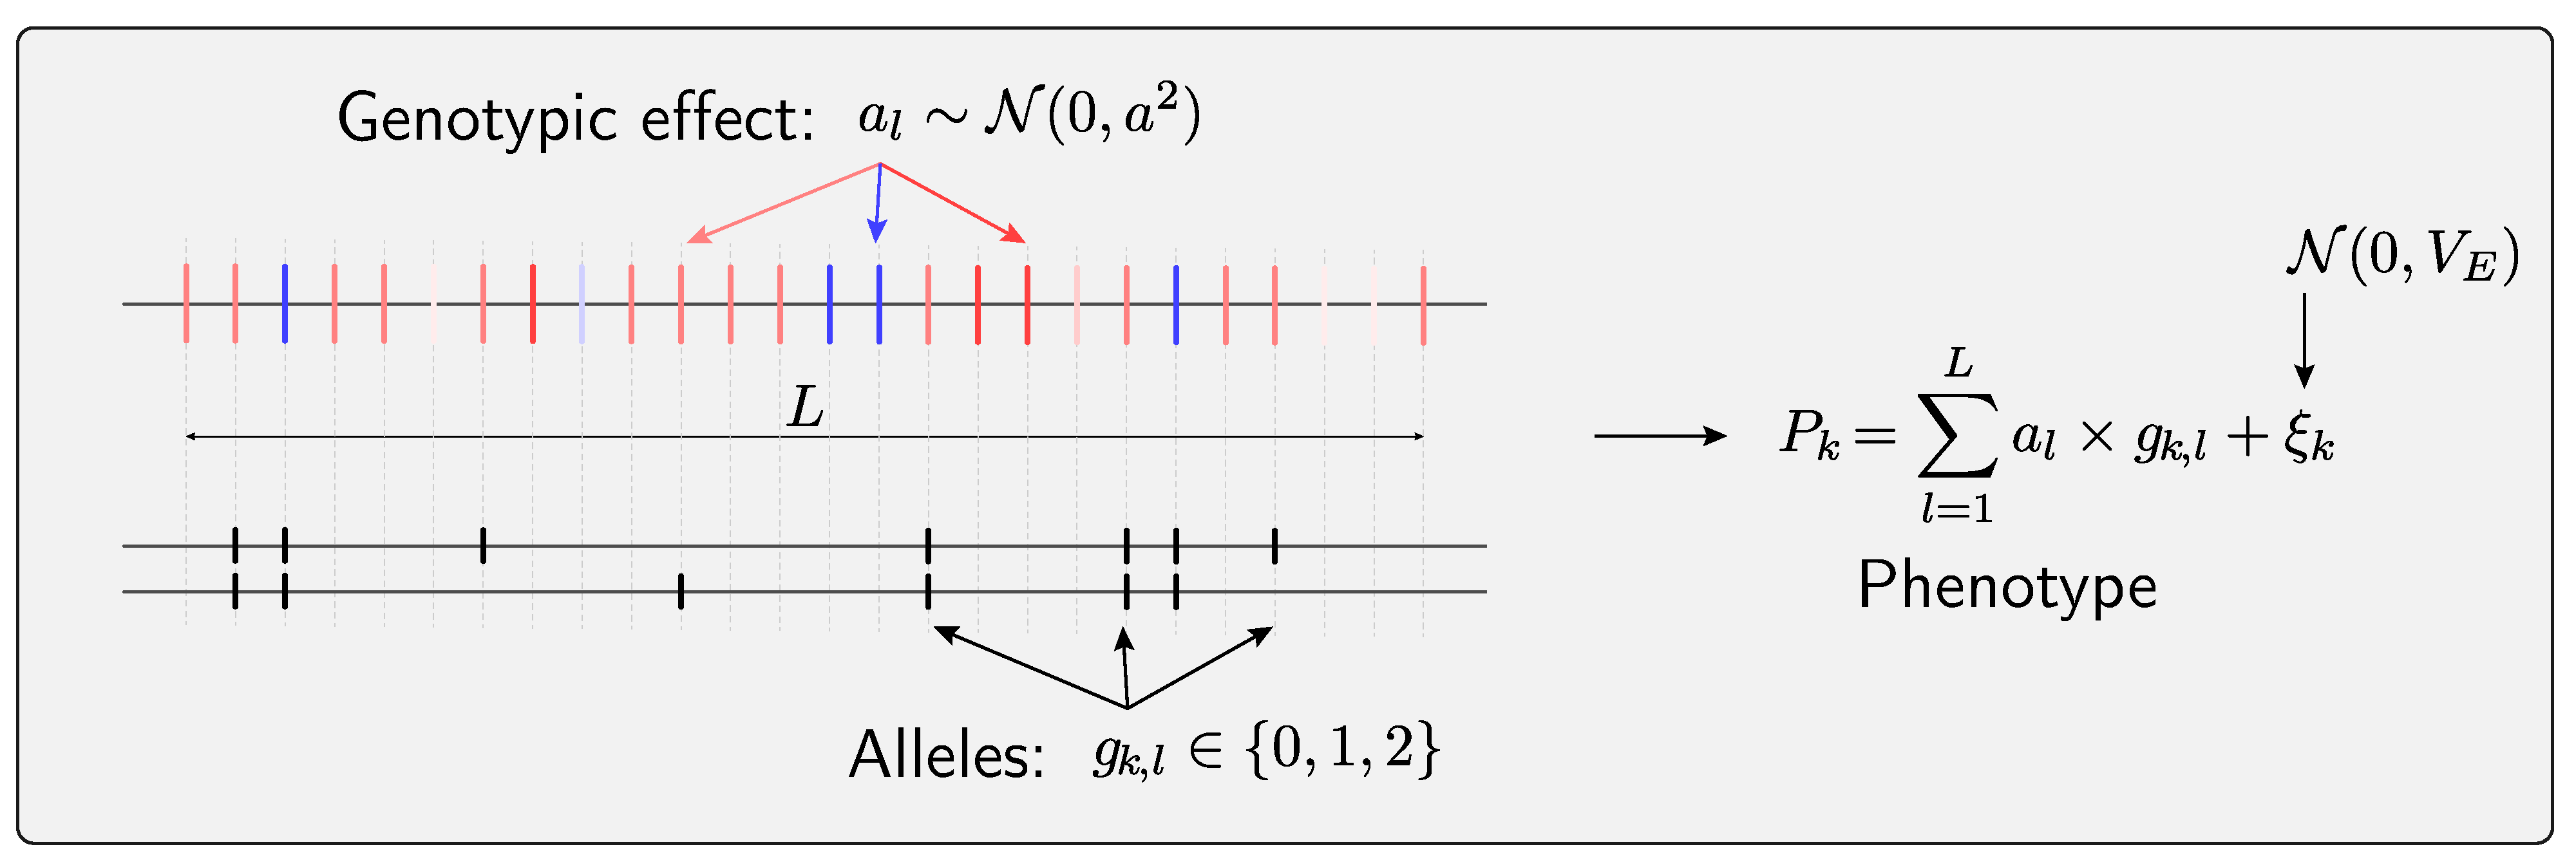
\includegraphics[width=0.6\textwidth, page=1] {figureS1}
    \label{fig:simulator-summary}
\end{center}

within-species, the mean ($\bar{G}$) and variance ($\VarGenetic$) of the genotype are:
\begin{equation}
    \bar{G} = \frac{1}{\Ne}\sum_{\Indiv=1}^{\Ne} G_{\Indiv} \text{\quad and \quad} \VarGenetic = \frac{1}{\Ne}\sum_{\Indiv=1}^{\Ne}\left(G_{\Indiv}- \bar{G} \right)^2\label{eq:simu-genotype}
\end{equation}
The theoretical additive genetic variance ($\VarGenetic$) is a function of the number of loci ($\NbrLoci$) and the effect of a mutation ($a$) as:
\begin{equation}
    \VarGenetic = 4 \Ne \Multiply \MutationRatePheno \Multiply \NbrLoci \Multiply a^2 \label{eq:simu-var-genetic}
\end{equation}

The mean ($\bar{\Trait}$) and variance ($\VarPhenotype$) of the phenotype are:
\begin{equation}
    \bar{\Trait} = \frac{1}{\Ne}\sum_{\Indiv=1}^{\Ne} \Trait_{\Indiv}\text{\quad and \quad} \VarPhenotype = \frac{1}{\Ne}\sum_{\Indiv=1}^{\Ne}\left(\Trait_{\Indiv} - \bar{\Trait} \right)^2 \label{eq:simu-between}
\end{equation}

Heritability ($\Heritability$) is defined as:
\begin{equation}
    \Heritability = \frac{\VarGenetic}{\VarPhenotype} = \frac{\VarGenetic}{\VarGenetic + \VarEnv}\label{eq:simu-heritability}
\end{equation}
Altogether, effective population size ($\Ne$), the number of loci ($\NbrLoci$) and the effect of a mutation ($a$), we can compute the variance of the environment ($\VarEnv$) that is required to reach a given heritability ($\Heritability$) as:
\begin{equation}
    \VarEnv = \VarGenetic \Multiply \left( \frac{1}{\Heritability} - 1 \right) = 4 \Ne \Multiply \MutationRatePheno \Multiply \NbrLoci \Multiply a^2 \Multiply \left( \frac{1}{\Heritability} - 1 \right) \label{eq:simu-var-env}
\end{equation}

\newpage
\section{Bayesian estimate}\label{sec:bayesian-estimate}

\subsection{Multivariate Brownian process}\label{subsec:multivariate-brownian-process}
Here we model $\Ntrait$ traits evolving along the phylogenetic tree that are correlated between them.
Their variation along the phylogeny is modeled as a $\Ntrait$-dimensional Brownian process $\Brownian$ ($1 \times \Ntrait$) starting at the root and branching along the tree topology.
The rate of change of the Brownian process is determined by the positive semi-definite and symmetric covariance matrix between traits $\CovarianceMatrix$ ($\Ntrait \times \Ntrait$).
Along branch $\Branch$ with length $d_{\Branch}$, the Brownian process start at the ancestral node $\mathcal{A}(\Branch)$ with value $\Brownian(\mathcal{A}(\Branch))$, and ends at node $\mathcal{R}(\Branch)$  with value $\Brownian(\mathcal{R}(\Branch))$.
The independent contrast $\contrast_{\Branch}$ defined as change in trait along the branch normalized by $\sqrt {d_{\Branch}}$ is a multivariate Gaussian:
\begin{equation}
    \label{eq:DistribBrownian}
    \contrast_{\Branch} = \frac{\Brownian (\mathcal{R}(\Branch)) - \Brownian (\mathcal{A}(\Branch)) }{\sqrt {d_{\Branch}}} \sim \mathcal{N}\left(\VecZero, \CovarianceMatrix \right).
\end{equation}

\subsection{Sampling the covariance matrix}\label{subsec:sampling-the-covariance-matrix}
From the independent contrast at each branch of the tree ($\contrast_{\Branch}$), we can define the $\Ntrait \times \Ntrait$ scatter matrix, $\Scattermatrix$, as:
\begin{equation}
    \Scattermatrix = \sum\limits_{\Branch=1}^{\Nbranch} \contrast_{\Branch} \MultiplyMatrix \contrast_{\Branch}\tr\label{eq:bayes-scatter},
\end{equation}
where $\Nbranch$ is the number of branches in the tree and $\NbrTaxa$ the number of taxa.

The {prior} on the covariance matrix is an inverse Wishart distribution, with $\Ntrait + 1$ degrees of freedom:
\begin{equation}
    \label{eq:Distribcovariance}
    \CovarianceMatrix \sim \text{Wishart}^{-1} (\Identitymatrix, \Ntrait + 1).
\end{equation}

By Bayes theorem, the {posterior} on $\CovarianceMatrix$, conditional on a particular realization of $\Brownian$ (and thus of $\contrast$) is an invert Wishart distribution, of parameter $\Identitymatrix + \Scattermatrix$ and with $\WishartPostDf$ degrees of freedom.
\begin{equation}
    \CovarianceMatrix \sim \text{Wishart}^{-1}\left( \Identitymatrix + \Scattermatrix, \WishartPostDf\right)\label{eq:bayes-posterior}
\end{equation}
This invert Wishart distribution can be obtained by sampling $\WishartPostDf$ independent and identically distributed multivariate normal random variables $\Multivariate_{\WishartIDD}$ defined by
\begin{equation}
    \Multivariate_{\WishartIDD} \sim \mathcal{N} \left( \VecZero, \left[ \Identitymatrix + \Scattermatrix\right]^{-1} \right).\label{eq:bayes-multivariate}
\end{equation}
And from these multivariate samples, $\CovarianceMatrix$ is Gibbs sampled as:
\begin{equation}
    \CovarianceMatrix = \left( \sum\limits_{\WishartIDD=1}^{\WishartPostDf} \Multivariate_{\WishartIDD} \MultiplyMatrix  \left[\Multivariate_{\WishartIDD} \right] \tr \right)\inv \label{eq:bayes-gibbs}
\end{equation}

\newpage
\section{Bayesian and Maximum-likelihood implementation}\label{sec:implementation}

Implementation is included within the \textit{BayesCode} software, available at \url{https://github.com/ThibaultLatrille/bayescode}.

\subsection{Data formatting}\label{subsec:data-formatting}

Running the analysis on your dataset and compute posterior probabilities requires three files:
\begin{enumerate}
    \item A phylogenetic tree in newick format, with branch lengths in number of substitutions per site (neutral markers), from which the values of nucleotide divergence ($d$) used in denominator of eq.~26 are used.
    \item A file containing the mean trait values for each species.
    \item A file containing the variation within-species for each trait and the genetic variation within-species (neutral markers).
\end{enumerate}

\subsubsection{Phylogenetic tree}

The phylogenetic tree must be in newick format, with branch lengths in substitutions per site (neutral markers).

\subsubsection{Mean trait for each species}

The file containing mean trait values for each species must be in a tab-delimited file with the following format:
\begin{center}
    \begin{adjustbox}{width = 0.35\textwidth}
        \begin{tabular}{|l|c|c|}
            \hline
            TaxonName            & Body\_mass & Brain\_mass \\
            \hline
            Panthera\_tigris     & 12.26      & 5.676       \\
            Pithecia\_pithecia   & 7.256      & 3.436       \\
            Colobus\_angolensis  & 9.176      & 4.284       \\
            Saimiri\_boliviensis & 6.845      & 3.279       \\
            $\vdots$             & $\vdots$   & $\vdots$    \\
            \hline
        \end{tabular}\label{tab:trait-mean}
    \end{adjustbox}
\end{center}

The columns are:
\begin{itemize}
    \item \emph{TaxonName}: the name of the taxon matching the name in the alignment and the tree.
    \item As many columns as traits, without spaces or special characters in the trait.
    \item The values can be \texttt{NaN} to indicate that the trait is not available for that taxon.
\end{itemize}

\newpage
\subsubsection{Trait variation for each species}

The file containing trait variation for each species must be in a tab-delimited file with the following format:
\begin{center}
    \begin{adjustbox}{width = 1.0\textwidth}
        \begin{tabular}{|l|c|c|c|c|c|c|}
            \hline
            TaxonName            & Nucleotide\_diversity & Body\_mass\_variance & Body\_mass\_heritability & Brain\_mass\_variance & Brain\_mass\_heritability \\
            \hline
            Pithecia\_pithecia   & 0.0016                & 0.22871              & 0.2                      & 0.00737               & 0.2                       \\
            Colobus\_angolensis  & 0.0017                & 0.00393              & 0.2                      & 0.00416               & 0.2                       \\
            Saimiri\_boliviensis & 0.0013                & 0.00022              & 0.2                      & 0.00045               & 0.2                       \\
            Pygathrix\_nemaeus   & 0.0016                & 0.00347              & 0.2                      & 0.00097               & 0.2                       \\
            $\vdots$             & $\vdots$              & $\vdots$             & $\vdots$                 & $\vdots$              & $\vdots$                  \\
            \hline
        \end{tabular}
        \label{tab:trait-variance}
    \end{adjustbox}
\end{center}

\begin{itemize}
    \item \emph{TaxonName}: the name of the taxon matching the name in the alignment and the tree.
    \item \emph{Nucleotide\_diversity}: the nucleotide diversity within-species (neutral markers), cannot be \texttt{NaN}.
    \item As many columns as traits, without spaces or special characters in the trait.
    \item \emph{TraitName\_variance}: the phenotypic variance of the trait within-species, can be \texttt{NaN} to indicate that the trait variance is not available for that taxon.
    \item \emph{TraitName\_heritability} (optional): the heritability of the trait within-species, between 0 and 1, cannot be \texttt{NaN}.
    \item The columns with the suffix \texttt{\_variance} and \texttt{\_heritability} are repeated for each trait.
    \item \emph{TraitName\_heritability\_lower} (optional): the lower bound of the heritability of the trait within-species, between 0 and 1, cannot be \texttt{NaN}.
    \item \emph{TraitName\_heritability\_upper} (optional): the upper bound of the heritability of the trait within-species, between 0 and 1, cannot be \texttt{NaN}.
    \item If the columns with the suffix \texttt{\_heritability\_lower} and \texttt{\_heritability\_upper} are present, the heritability is randomly drawn from a uniform distribution between the lower and upper bounds.
    \item If the columns with the suffix \texttt{\_heritability} is present, it is taken as is.
    \item If the additive genetic variance (instead of phenotypic variance) is available for a trait, the heritability can be omitted and will automatically be set to 1.0.
\end{itemize}

\newpage
\subsection{Bayesian estimation}\label{subsec:running-nodetraitsand-readnodetraits}

The executable \texttt{nodetraits} from \textit{BayesCode} is used to run the Bayesian estimation of the model, and the executable \texttt{readnodetraits} is used to read the results.

Assuming that the file \texttt{data/body\_size/mammals.male.tsv} contains the mean trait values for each species, the file \texttt{data/body\_size/mammals.male.var\_trait.tsv} contains the variation within-species for each trait and the genetic variation within-species (neutral markers), and the file \texttt{data/body\_size/mammals.male.tree} contains the phylogenetic tree, the following commands are used to run the model and read the results.

\subsubsection{Running the model}
\texttt{nodetraits} is run with the following command:
\begin{lstlisting}[language = sh,label={lst:nodetraits-run}]
nodetraits  --until 2000
            --tree data/body_size/mammals.male.tree
            --traitsfile data/body_size/mammals.male.tsv
            run_mammals_male
\end{lstlisting}

\subsubsection{Reading the results}
Once the model has run, the chain \texttt{run\_mammals\_male} is used to compute the posterior distribution of the ratio of between-species variation over within-species variation with \texttt{readnodetraits}:
\begin{lstlisting}[language = sh,label={lst:readnodetraits-rho}]
readnodetraits --burnin 1000
               --var_within data/body_size/mammals.male.var_trait.tsv
               --output results_mammals_male.tsv
               run_mammals_male
\end{lstlisting}
The file \texttt{data\_empirical/chain\_name.ratio.tsv} then contains the posterior mean of the ratio of between-species variation over within-species variation, the 95\% and 99\% credible interval, and the posterior probability that the ratio is greater than 1.

\subsection{Maximum likelihood estimation}\label{subsec:maximum-likelihood-estimation}

To obtain the ratio (without the posterior credible interval and probability) using maximum likelihood computation, the following python script can be used:
\begin{lstlisting}[language = sh, label={lst:neutrality_index}]
python3 utils/neutrality_index.py --tree data/body_size/mammals.male.tree
                                  --traitsfile data/body_size/mammals.male.tsv
                                  --var_within data/body_size/mammals.male.var_trait.tsv
                                  --output results_ML_mammals_male.tsv
\end{lstlisting}

\newpage
\section{Saturation of phenotypic divergence}\label{sec:supp-distance}

In our simulation setting, the genetic architecture underlying the phenotype is not changing along the phylogeny.
As a result, the phenotype may be bounded by what such genetic architecture can produce, and this could cause a slowdown of phenotypic divergence over time, ultimately resulting in a decreased $\RateBetween$.

\begin{center}
    \captionof{figure}{Saturation of phenotypic divergence.}
    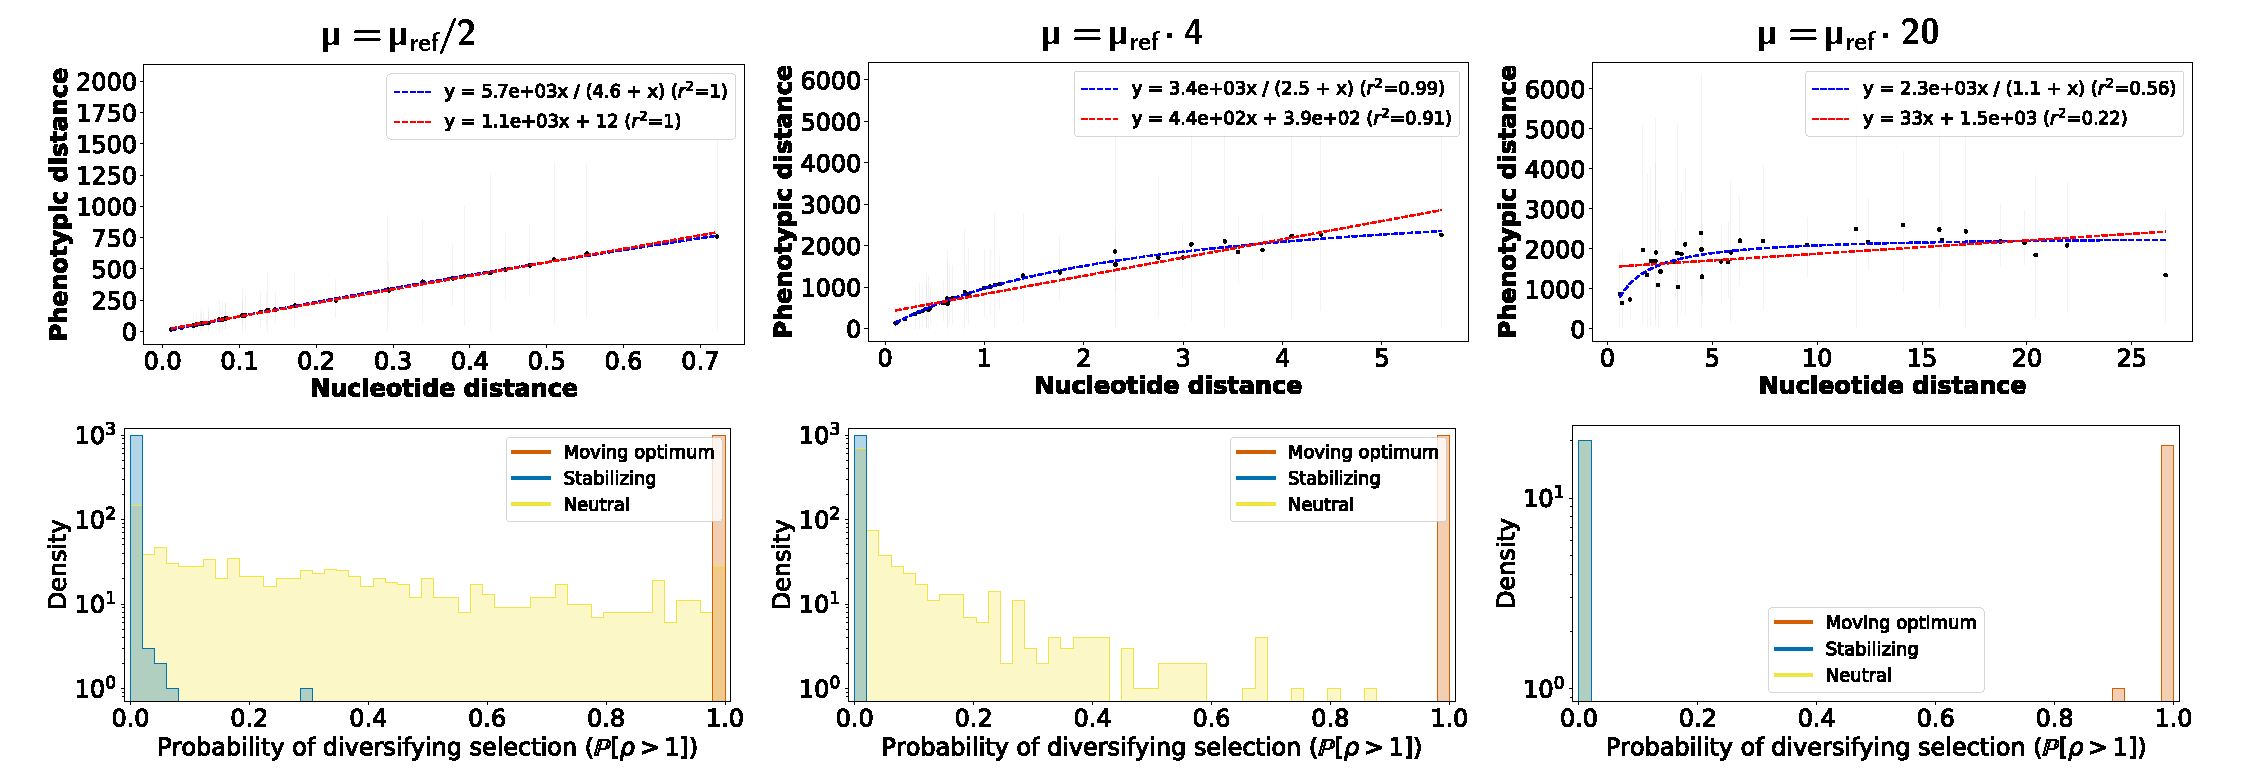
\includegraphics[width=1.0\textwidth, page=1] {figureS2}
    \label{fig:supp-distance}
\end{center}
\begin{itemize}
    \item Left column: $1,000$ simulations with low divergence between species (half that of mammals).
    \item Middle column: $1,000$ simulations with high divergence between species (4 times that of mammals).
    \item Right column: $200$ simulations with very high divergence between species (20 times that of mammals).
    \item Top row: Simulation of neutral trait, phenotypic divergence between species as a function of the nucleotide divergence. Phenotypic divergence is computed between two species as the covariance between the trait ($\VarPhy$), and the nucleotide divergence is computed as the number of substitutions per site shared between the two species ($d$). Each point is a pair of species, and the bounds of the intervals in grey are the 2.5\% and 97.5\% quantiles across the replicates. The blue line is the linear regression and the red line is the saturation model ($y = \alpha \Multiply x / (\beta + x)$).
    \item Bottom row: Traits simulated under stabilizing selection (blue), under a neutral evolution (yellow), and under a moving optimum (red). Histogram of probabilities of $\NI$ being greater than $1$.
\end{itemize}
Under a model of neutral trait evolution, when mutation rate increases, or equivalently the divergence between species increases, the phenotypic divergence between species saturates faster than the nucleotide divergence.
This saturation effect can result in a spurious signal of stabilizing selection ($\NI < 1$) for deeper phylogeny when the trait is evolving neutrally.
\end{document}
%TC:endignore